\chapter{Six Questions With a Public CEO}

This chapter follows a School of Hard Knocks interview with Mark White, curated by LazyingArt LLC through Video2Book. The source is not a blackboard lecture, and there are no validated board screenshots to preserve. Its serious structure is commercial rather than formal-physical: we will keep the interview's order, separate anecdote from claim, and express the repeatable parts as small mechanisms that can be inspected.

\section{The Opening Frame: Why This Witness Matters}

James Newman begins by telling us why Mark White is being treated as a witness worth listening to. White is introduced as the CEO of a public company, associated here with Nexalyn Technologies, and as someone who runs a business concerned with mental health, psychiatric medication, and frequencies. The host then moves from status to purpose: White has invited the show to his Houston headquarters to offer young entrepreneurs more practical game.

That opening creates the first useful tension. We are not beginning with a theory of wealth or a financial model. We are beginning with a person who has reached a public-company role, and then asking what had to be learned before that title meant anything. For these notes, the object we track is therefore not an equation of physics but a disciplined unit of judgment:
\begin{equation}
\text{lesson}
=
\text{anecdote}
+
\text{speaker's claim}
+
\text{portable mechanism}.
\end{equation}
The anecdote fixes the lesson to the source. The claim records what White believes the event means. The mechanism is the part we can test in another business, another room, or another failure.

\section{First Money: A Valet Job Becomes a Service Business}

The first direct question is clean: what was the first business he ever started? White answers, ``car detailing,'' and then reconstructs the scene. He was a valet parker at a Houston hotel during the late-1970s oil boom, near the new Galleria, when many nice restaurants were still inside hotels. Customers drove in, handed over the car, and went to dinner.

Before any formal company existed, White had three ingredients: temporary access to the car, idle time while the owner ate, and a visible improvement he could make. Armor All was new. Cleaning a wheel and treating a tire could make the car look newly refreshed. White and the doorman turned that into a small offer: while the customer was at dinner, they would wash and detail the car. The price he names is \(\$20\).

\subsection{Question \& Answer}

\paragraph{Question.} What was the first real money-making mechanism?

\paragraph{Answer.} It was controlled access plus visible proof. The customer had already trusted the valet with the car. Dinner created the time window. Armor All created the before-and-after effect. The \(\$20\) offer made the trial small enough to accept.

A compact reconstruction is:
\begin{equation}
\text{Opportunity}
\approx
\text{access}
+
\text{idle time}
+
\text{visible improvement}
+
\text{small offer}.
\end{equation}
This is not a formula spoken in the interview. It is the mechanism made explicit.

The operation then became repeatable. White says he parked cars at night and, in the mornings, picked up Lincoln Mark Fives and Cadillac Eldorados from customers' offices, took them to his house, cleaned the wheels with a toothbrush, and Armor Alled the tires. The business began inside a small constraint and expanded because the proof was visible.

\begin{figure}
\centering
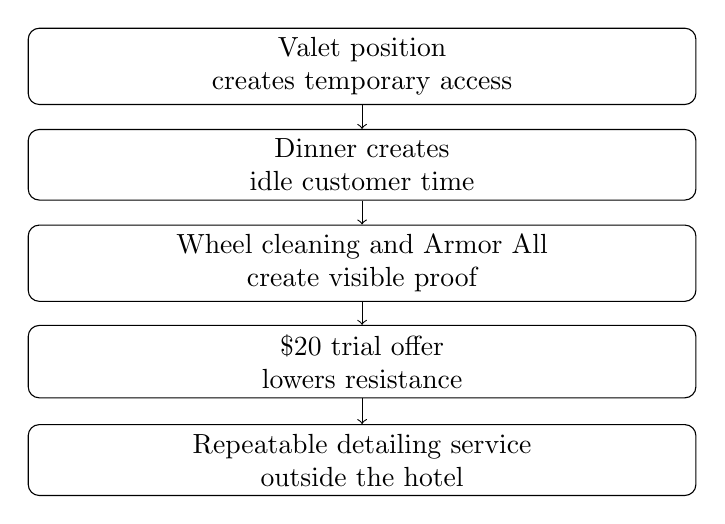
\begin{tikzpicture}
\node[draw, rounded corners, align=center, text width=.68\linewidth] (a) at (0,0) {Valet position\\creates temporary access};
\node[draw, rounded corners, align=center, text width=.68\linewidth] (b) at (0,-1.25) {Dinner creates\\idle customer time};
\node[draw, rounded corners, align=center, text width=.68\linewidth] (c) at (0,-2.50) {Wheel cleaning and Armor All\\create visible proof};
\node[draw, rounded corners, align=center, text width=.68\linewidth] (d) at (0,-3.75) {\(\$20\) trial offer\\lowers resistance};
\node[draw, rounded corners, align=center, text width=.68\linewidth] (e) at (0,-5.00) {Repeatable detailing service\\outside the hotel};
\draw[->] (a) -- (b);
\draw[->] (b) -- (c);
\draw[->] (c) -- (d);
\draw[->] (d) -- (e);
\end{tikzpicture}
\caption{A transcript-grounded reconstruction of the first-business mechanism.}
\end{figure}

\section{Sales as Communication Rather Than Pressure}

The host then pivots naturally: if the first business required strangers to say yes, what was White's secret to sales? White acknowledges the sales-training culture of his era, naming Zig Ziglar and Tony Robbins, but he does not place his own method under the heading of hard closing. His answer is communication.

He says he has energy, confidence, and has learned how to communicate. More importantly, he says great salespeople are often not ``salesmen'' or ``saleswomen'' in the narrow sense. They are people who love their product or service, believe in it, and communicate that belief. When he talks about Nexalyn technology, mind care, brain training, or brain stimulation, he expects the listener to see that he loves what he does. That creates what he calls a natural sales moment.

\subsection{Question \& Answer}

\paragraph{Question.} What is the selling move beneath the enthusiasm?

\paragraph{Answer.} White's move is to enter the room by asking why the buyer might say no. That question changes the sales problem. The seller is no longer merely reciting a pitch; he is searching for the buyer's obstacle.

The loop is:
\begin{equation}
\text{Ask}
\longrightarrow
\text{Listen}
\longrightarrow
\text{Tailor}
\longrightarrow
\text{Respect}
\longrightarrow
\text{Engage}.
\end{equation}
He asks questions, listens to the response, and tailors the message to the buyer's needs. The respect term is essential. White says he does not want to tell people what they do not want to know, nor tell them something they already know better than he does.

That is why the sales section leads directly to humility. In a room of medical professionals, White's first move is not to pretend he knows healthcare better than they do. It is to acknowledge the room's expertise and offer, in his words, a vision of what he thinks could be a better healthcare system.

\section{Mentor Advice: Fewer Words, Money Discipline, Humility}

The host next asks for the best advice White ever received from a mentor. White's first answer is almost corrective: talk too much; slow down; say what you are going to say in fewer words, because the people listening do not know it as well as you know it.

Then he moves to money. In entrepreneurial life, he says, personal and professional finances come together. A company has a big week, a few thousand dollars come in, and suddenly the founder is buying a suit at Saks Fifth Avenue or a \(\$200\) bottle of wine. The point is not that a single purchase destroys an enterprise. The point is that a founder's personal appetite can leak out of the same reservoir that the business needs.

\begin{equation}
\text{business cash}
+
\text{personal spending impulse}
\longrightarrow
\text{capital leakage}.
\end{equation}

\subsection{Question \& Answer}

\paragraph{Question.} How can an aggressive entrepreneur remain humble?

\paragraph{Answer.} White distinguishes confidence from pretending. He says he is confident and aggressive, but tries to stay aware of what he does not know. Humility becomes a constraint on behavior: speak in fewer words, do not spend as if every good week is permanent, and do not outrank the expert in the room.

He also gives a useful distinction:
\begin{align}
\text{knowledge} &\approx \text{firsthand experience},\\
\text{wisdom} &\approx \text{listening to those with knowledge}.
\end{align}
That distinction is a hinge in the interview. We move from skill and selling into a larger claim about how a person learns without becoming overconfident.

\section{Trauma and the Claimed Two-System Model of the Brain}

The host then changes terrain. He brings up Kanye West as a public example of someone with a close relationship to his mother, followed by public controversy, concern about mental health, medication, and weight gain. The question becomes: how can relationship trauma affect the brain?

White begins by broadening the word trauma. In his framing, trauma is not only a major injury. It is anything abnormal in day-to-day life experience. He names three main forms:
\begin{equation}
\text{Trauma}
=
\{\text{toxic},\ \text{physical},\ \text{emotional}\}.
\end{equation}
Toxic trauma includes addiction, alcohol, drugs, food sensitivity, and poisons. Physical trauma includes football injuries, falls, head injuries, traumatic brain injury, and war injuries. Emotional trauma includes loss of a loved one and betrayal by a loved one.

\subsection{Question \& Answer}

\paragraph{Question.} How does relationship trauma affect the brain, according to White?

\paragraph{Answer.} White's attributed model is that the brain has two systems, an electrical system and a chemical system, and that trauma can disturb one or both. He describes the systems as doing a dance. Their job, in his language, is to help a person handle life on life's terms.

We record the claim cautiously:
\begin{equation}
\text{brain system}
=
\text{chemical system}
+
\text{electrical system}.
\end{equation}
The next step in his account is fight or flight. During a traumatic event, the brain protects the person. Afterward, the system may not return cleanly to balance. White then brings in PTSD, emphasizing that he does not restrict it to military experience. In his examples, it may follow a bad marriage, a bad employer, or the loss of a loved one.

His claimed manifestation channels are:
\begin{equation}
\text{trauma response}
\longrightarrow
\{\text{chemical imbalance},\ \text{EEG/frequency disturbance}\}.
\end{equation}
He names dopamine, serotonin, and acetylcholine on the chemical side, and EEG or frequencies on the electrical side. These notes preserve the claim as White's model. They do not turn it into independent medical proof.

\subsection{Treatment Claims and Caution}

White then argues that psychiatric treatment can sometimes become, in his phrase, a guessing game. A patient reports depression, lost desire, or a deteriorating marriage; a medication such as Prozac is tried; and the attempt is to chemically alter a brain that White already describes as chemically altered. He says this may work some of the time, but not all of the time.

His preferred starting point is also a claim, not a demonstrated result in the transcript: begin with non-invasive technologies, nutrition improvements, talk therapy or conversation with a trusted person, and the foundations of life. He also says that, as a man of faith, he believes in belonging to a spiritual community.

The practical rhythm of the answer is gradualism. You do not get into a condition overnight, and you do not get out overnight. His analogy is weight: one does not gain a hundred pounds overnight and should not expect to lose a hundred pounds overnight. This idea will return in the final self-improvement section.

\section{Failure as the Greatest Accomplishment}

The host returns to entrepreneurship: White has started companies and brought a company public, so what is his greatest accomplishment? The expected answer might be the public company. White gives the reversal: getting up, brushing himself off, licking his wounds, and going back in for another round.

He says the worst thing after never having money is having a lot of money, losing it, and then not having any money. The central image is severe: watching his life's work get loaded into trucks and taken down the road. He names a bankruptcy attorney, rendered in the transcript as Nelson Hemsley, who gave him a choice. White could pay the attorney to go to court and clean up the mess, or he could come to every meeting, go to the courthouse, and face the people he owed money to.

\subsection{Question \& Answer}

\paragraph{Question.} Why is failure, rather than going public, named as the greatest accomplishment?

\paragraph{Answer.} Because the failure forced accountability. White says his greatest accomplishment was having the strength and nerve to enter a room of people who hated him because he had failed, owed them money, and they lost money. He presents this not as a slogan but as a brutal education.

The mechanism is:
\begin{equation}
\text{failure}
+
\text{creditor-facing accountability}
+
\text{humility}
\longrightarrow
\text{practical wisdom}.
\end{equation}

The ordered lesson is:
\begin{enumerate}
\item A business failure creates obligations to real people.
\item Avoidance may preserve comfort, but it forfeits the lesson.
\item Facing creditors converts failure into accountability.
\item Giving assets back and watching them be sold imposes humility.
\item On the other side, White says he became a new man.
\end{enumerate}

That last phrase includes more than business. White says he gained a new level of respect for his fellow man, remarried his wife, put his family back together, and learned humility. The repeated word matters. Humility is not a decorative virtue in this interview; it is the mechanism by which pain becomes usable judgment.

\section{Structure as Self-Improvement}

The final turn is deliberately practical. The host asks whether White reads. White says he is not a reader; he is a skimmer. Then the host asks for self-improvement advice for people who are out of shape, distracted by Netflix and dopamine, and trying to become serious about their lives.

White answers with one word: structure.

He tells a story about a man named Haas. Haas told him to set an alarm for 8 a.m., get out of bed, make the bed, shower, be ready at 9 a.m., eat lunch at noon, eat dinner at six, prepare for bed at night, and get in bed. White's response was: that's it? Haas's answer was the point: you need to be successful at something.

We can model this as a small update rule for self-trust. Let \(S_n\) denote a bookkeeping measure of self-trust after \(n\) days. It is not a clinical variable; it is a simple way to make White's mechanism explicit.
\begin{align}
S_{n+1} &= S_n + \delta,
\qquad \delta > 0
\quad \text{if today's promise is kept},\\
S_{n+1} &= S_n - \epsilon,
\qquad \epsilon > 0
\quad \text{if today's promise is abandoned}.
\end{align}
The point is not the numerical value. The point is that a small kept promise supplies evidence. At the end of the day, the person can sit quietly and notice: I did what I said I would do.

\subsection{A Worked Example}

Suppose the only promise is this: wake at 8 a.m., make the bed, and be on time to work. Let \(S_0=0\). Suppose a kept promise adds \(1\) unit and a broken promise subtracts \(2\) units. For five days with the pattern
\[
\text{kept},\quad
\text{kept},\quad
\text{broken},\quad
\text{kept},\quad
\text{kept},
\]
we get
\begin{align}
S_1 &= 0+1=1,\\
S_2 &= 1+1=2,\\
S_3 &= 2-2=0,\\
S_4 &= 0+1=1,\\
S_5 &= 1+1=2.
\end{align}
The numbers are illustrative, but the direction is faithful to the answer. A person does not rebuild by announcing a total transformation. He rebuilds by choosing a promise small enough to keep, keeping it, noticing the kept promise, and repeating.

White contrasts this with the New Year's resolution pattern. A person tries to stop A, B, C, D and start E, F, G, H all at once. He gets through A and B, fails, feels ashamed, turns on Netflix, gets chips, and starts over. The correction is a smaller unit of success.

\begin{figure}
\centering
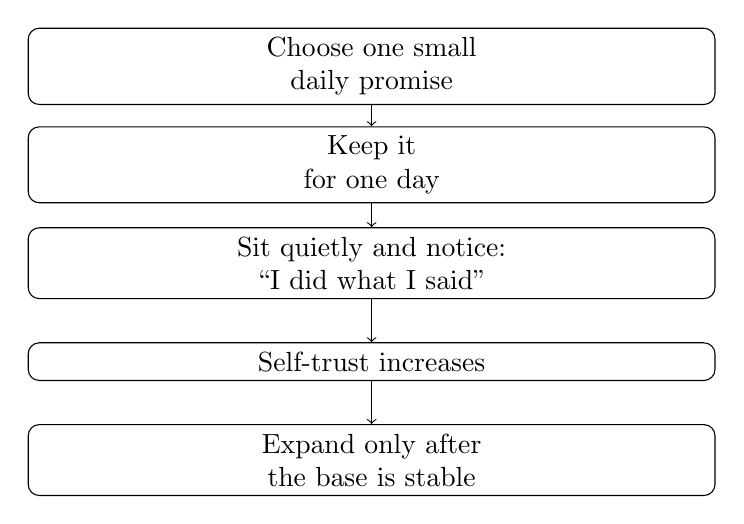
\begin{tikzpicture}
\node[draw, rounded corners, align=center, text width=.70\linewidth] (a) at (0,0) {Choose one small\\daily promise};
\node[draw, rounded corners, align=center, text width=.70\linewidth] (b) at (0,-1.25) {Keep it\\for one day};
\node[draw, rounded corners, align=center, text width=.70\linewidth] (c) at (0,-2.50) {Sit quietly and notice:\\``I did what I said''};
\node[draw, rounded corners, align=center, text width=.70\linewidth] (d) at (0,-3.75) {Self-trust increases};
\node[draw, rounded corners, align=center, text width=.70\linewidth] (e) at (0,-5.00) {Expand only after\\the base is stable};
\draw[->] (a) -- (b);
\draw[->] (b) -- (c);
\draw[->] (c) -- (d);
\draw[->] (d) -- (e);
\end{tikzpicture}
\caption{A transcript-grounded reconstruction of the small-promise structure.}
\end{figure}

The closing advice is to start small and get honest. White asks the listener to identify the Achilles heel: sugar, vodka, marijuana, a bad marriage, meanness to people, or some other pattern. Then choose one action. Say hello to everybody and smile. Do that today. At the end of the day, the person feels a small but real difference.

\section{Summary}

The interview begins with the authority of a public CEO, but its durable lessons come from smaller scenes: a valet sees a \(\$20\) detailing opportunity; a salesman asks why the buyer might say no; a founder learns not to let business income leak into personal display; a health entrepreneur describes trauma through his own two-system model; a failed businessman faces creditors; and a struggling person rebuilds from one kept promise.

The common structure is attention to mechanisms. Access can become opportunity. Communication can replace pressure. Humility can protect judgment. Failure can become education when it is faced directly. Structure can rebuild self-trust when it begins small enough to keep.